\documentclass[12pt]{article}
\usepackage{preamble}

\begin{document}

\begin{titlepage}

    \begin{tikzpicture}[remember picture, overlay]
        \draw[line width = 1pt] ($(current page.north west) + (1cm,-1cm)$) rectangle ($(current page.south east) + (-1cm,1cm)$);
    \end{tikzpicture}

   \begin{center}
        \Large{\textbf{\subject}} \\
        \vspace{0.5cm}
        \large{University of Colombo School of Computing}

        \vspace{1.5 cm}

        \Huge{\textbf{\titleofdoc}} \\
        % \Large{\slogan} \\

        \vspace{1cm}
        \LARGE{\subtitleofdoc}
            

        \vspace{1.5 cm}
        \Large{\textbf{\group}} \\
        
        \vspace{0.9 cm}
        \begin{tabular}{|l|l|}
            \hline
            \normalsize Name & \normalsize Index Number \\
            \hline
            \small WIJEGUNAWARDANE I.A.P.P. & \normalsize 20002157 \\
            \hline
            \small WICKRAMASINGHE W.M.O.E. & \normalsize 20002149 \\
            \hline
            \small WALGAMA R.R. & \normalsize 20001959 \\
            \hline
            \small PERERA M.A.I.A. & \normalsize 20001304 \\
            \hline
            \small DE SILVA T.P.M. & \normalsize 20000375 \\
            \hline
            \small HARISCHANDRA L.I.L. & \normalsize 20000715 \\
            \hline
            \small SAMALIARACHCHI H.U. & \normalsize 20001551 \\
            \hline
        \end{tabular}

        \vspace{2 cm}
        \Large{\today}
        
        \vspace{0.25 cm}
       \vfill
    \end{center}
\end{titlepage}

\setcounter{page}{2}
\pagestyle{fancy}
\fancyhf{}
\lhead{\color{gray}{\nouppercase{\leftmark}}}
% \lfoot{\color{gray}{\titleofdoc: \slogan}}
% \rhead{\color{gray}{\Author : \indexno}}
\rfoot{\color{gray}{\thepage}}
\pagenumbering{Roman} 

\newpage

\tableofcontents

\listoffigures
% \listoftables

\newpage
\pagenumbering{arabic} 


\section{Introduction to the Solution} 
Sri Tel Ltd (STL), a Sri Lankan-based telecommunication company, aims to enhance its market share by focusing on improving customer care and customer experience. As part of this initiative, STL plans to introduce a state-of-the-art Internet-based Customer Care Web Portal which is implemented using a React web app that can be scalable with platform-independent solutions such as Android and iOS with provided microservices-based APIs. The solution empowers customers to configure and pay for their services independently through a payment gateway. Key functionalities include account creation, bill payments, service activations, bill viewing, notifications, and online chat support. This report contains a comprehensive analysis of the architecture of this requirement and provides the implementation of a Spring Boot application with a scalable architecture.

\section{Architecture of the Solution}
\begin{figure}[ht]
    \centering
    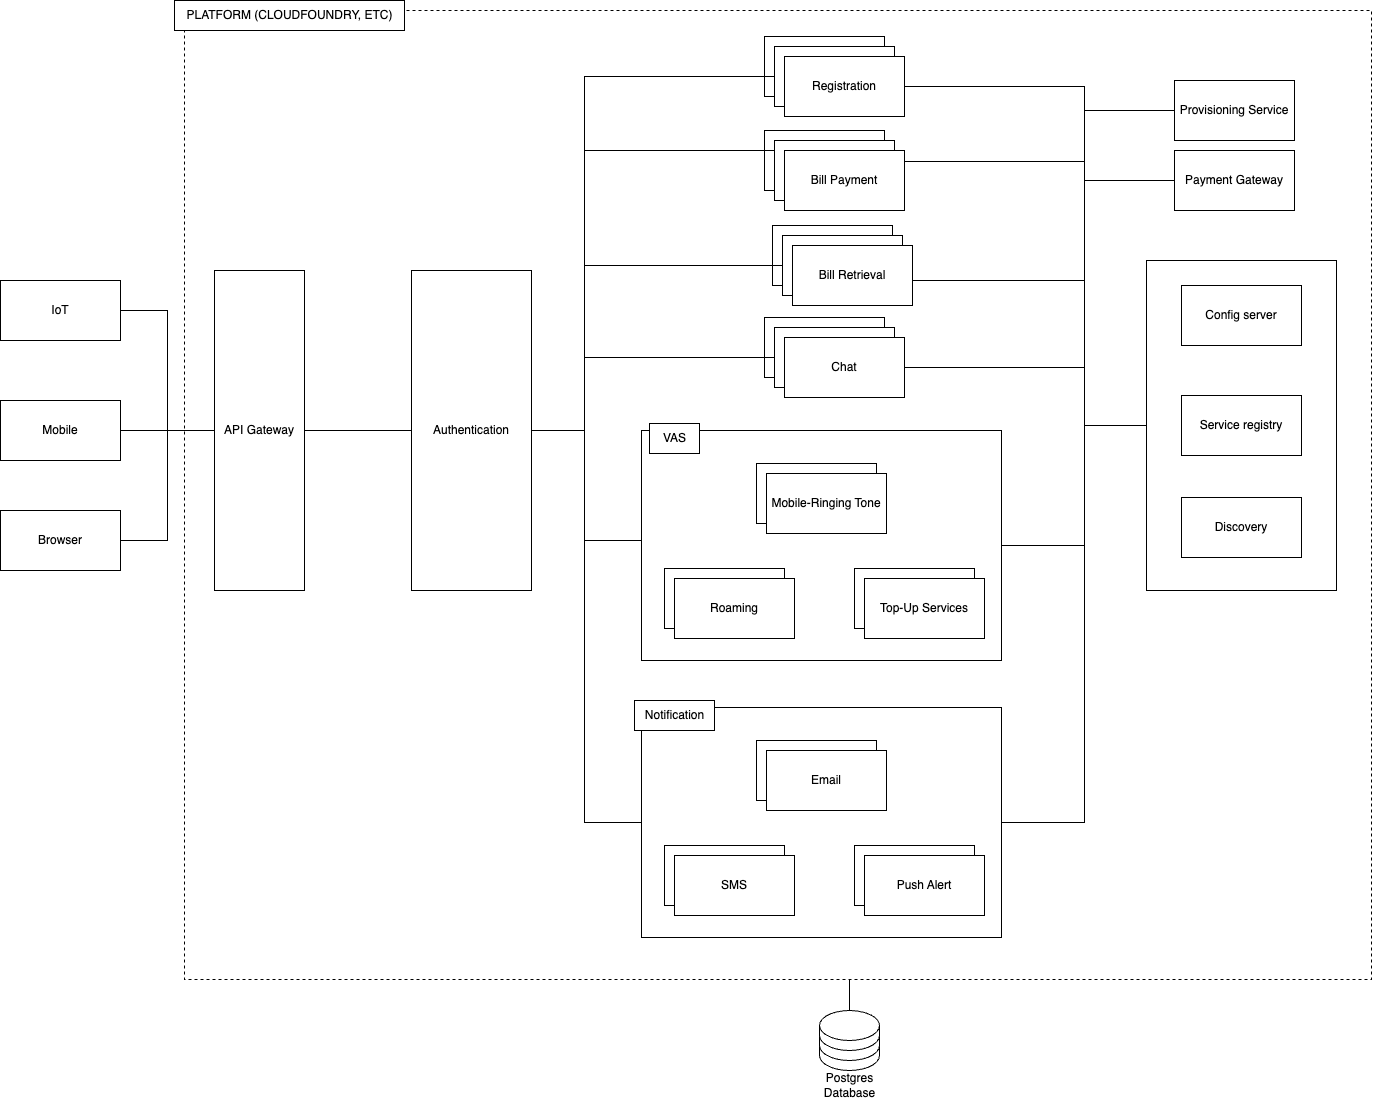
\includegraphics[width=\linewidth]{Architecture.png}
    \caption{Proposed Microservices Architecture.}
    \label{fig:your-figure-label}
\end{figure}

The Sri-Tel Ltd solution encompasses the following components:
\begin{itemize}
    \item \textbf{User Management}: This component is responsible for user account creation, and email-password-based login. It should be simple and secure, allowing users to create accounts without manual assistance.
    \item \textbf{Billing and Payment}: Manages bill generation, bill viewing, and online payment processing using credit and debit cards.
    \item \textbf{Service Activation/Deactivation}: Interfaces with the existing Provisioning System to activate or deactivate Telco services, including Value Added Services (VAS), voice, and data services.
    \item \textbf{Notification Engine}: Delivers email, SMS, and push alerts to customers based on bill generation, service issues, disconnections, and other relevant events. It should not hinder the primary functions of the solution.
    \item \textbf{Online Chat Support}: Facilitates real-time chat between customers and customer care agents for issue resolution. 
\end{itemize}

\par The proposed solution architecture is based on the Eureka server implemented using Spring Boot. In a Spring Boot microservices architecture, an API Gateway acts as a single entry point for all client requests, routing them to the appropriate microservice. Users have to first login in which is implemented as a service. 

\par The proposed system consists of a configuration server and a service registry to look up and register services which are connected to all the available services. Hence it should not be a single point of failure; should be highly available. The service discovery is responsible for discovering new services and handling them. 

\par The VAS is implemented as a Mobile Ringing Tone with Roaming features and Top-up services where users can add them as they wish using the web interface. Notifications service is described as Email, SMS, and Push Alert notifications. This will be communicated to the user through the application where the user can select each from the dashboard.

\par The provided API is configurable with a mobile, IoT, or any other application since the provided implementation is done using REST-full API. The implementation has been done only on the web for demonstration easiness.

\par Postgres database is used as the database with a single database to mimic the data source and it is running on the default port 5432. Below is shown the Eureka server with all the service statuses when all the services are running.

\newpage    

\begin{figure}[H]
    \centering
    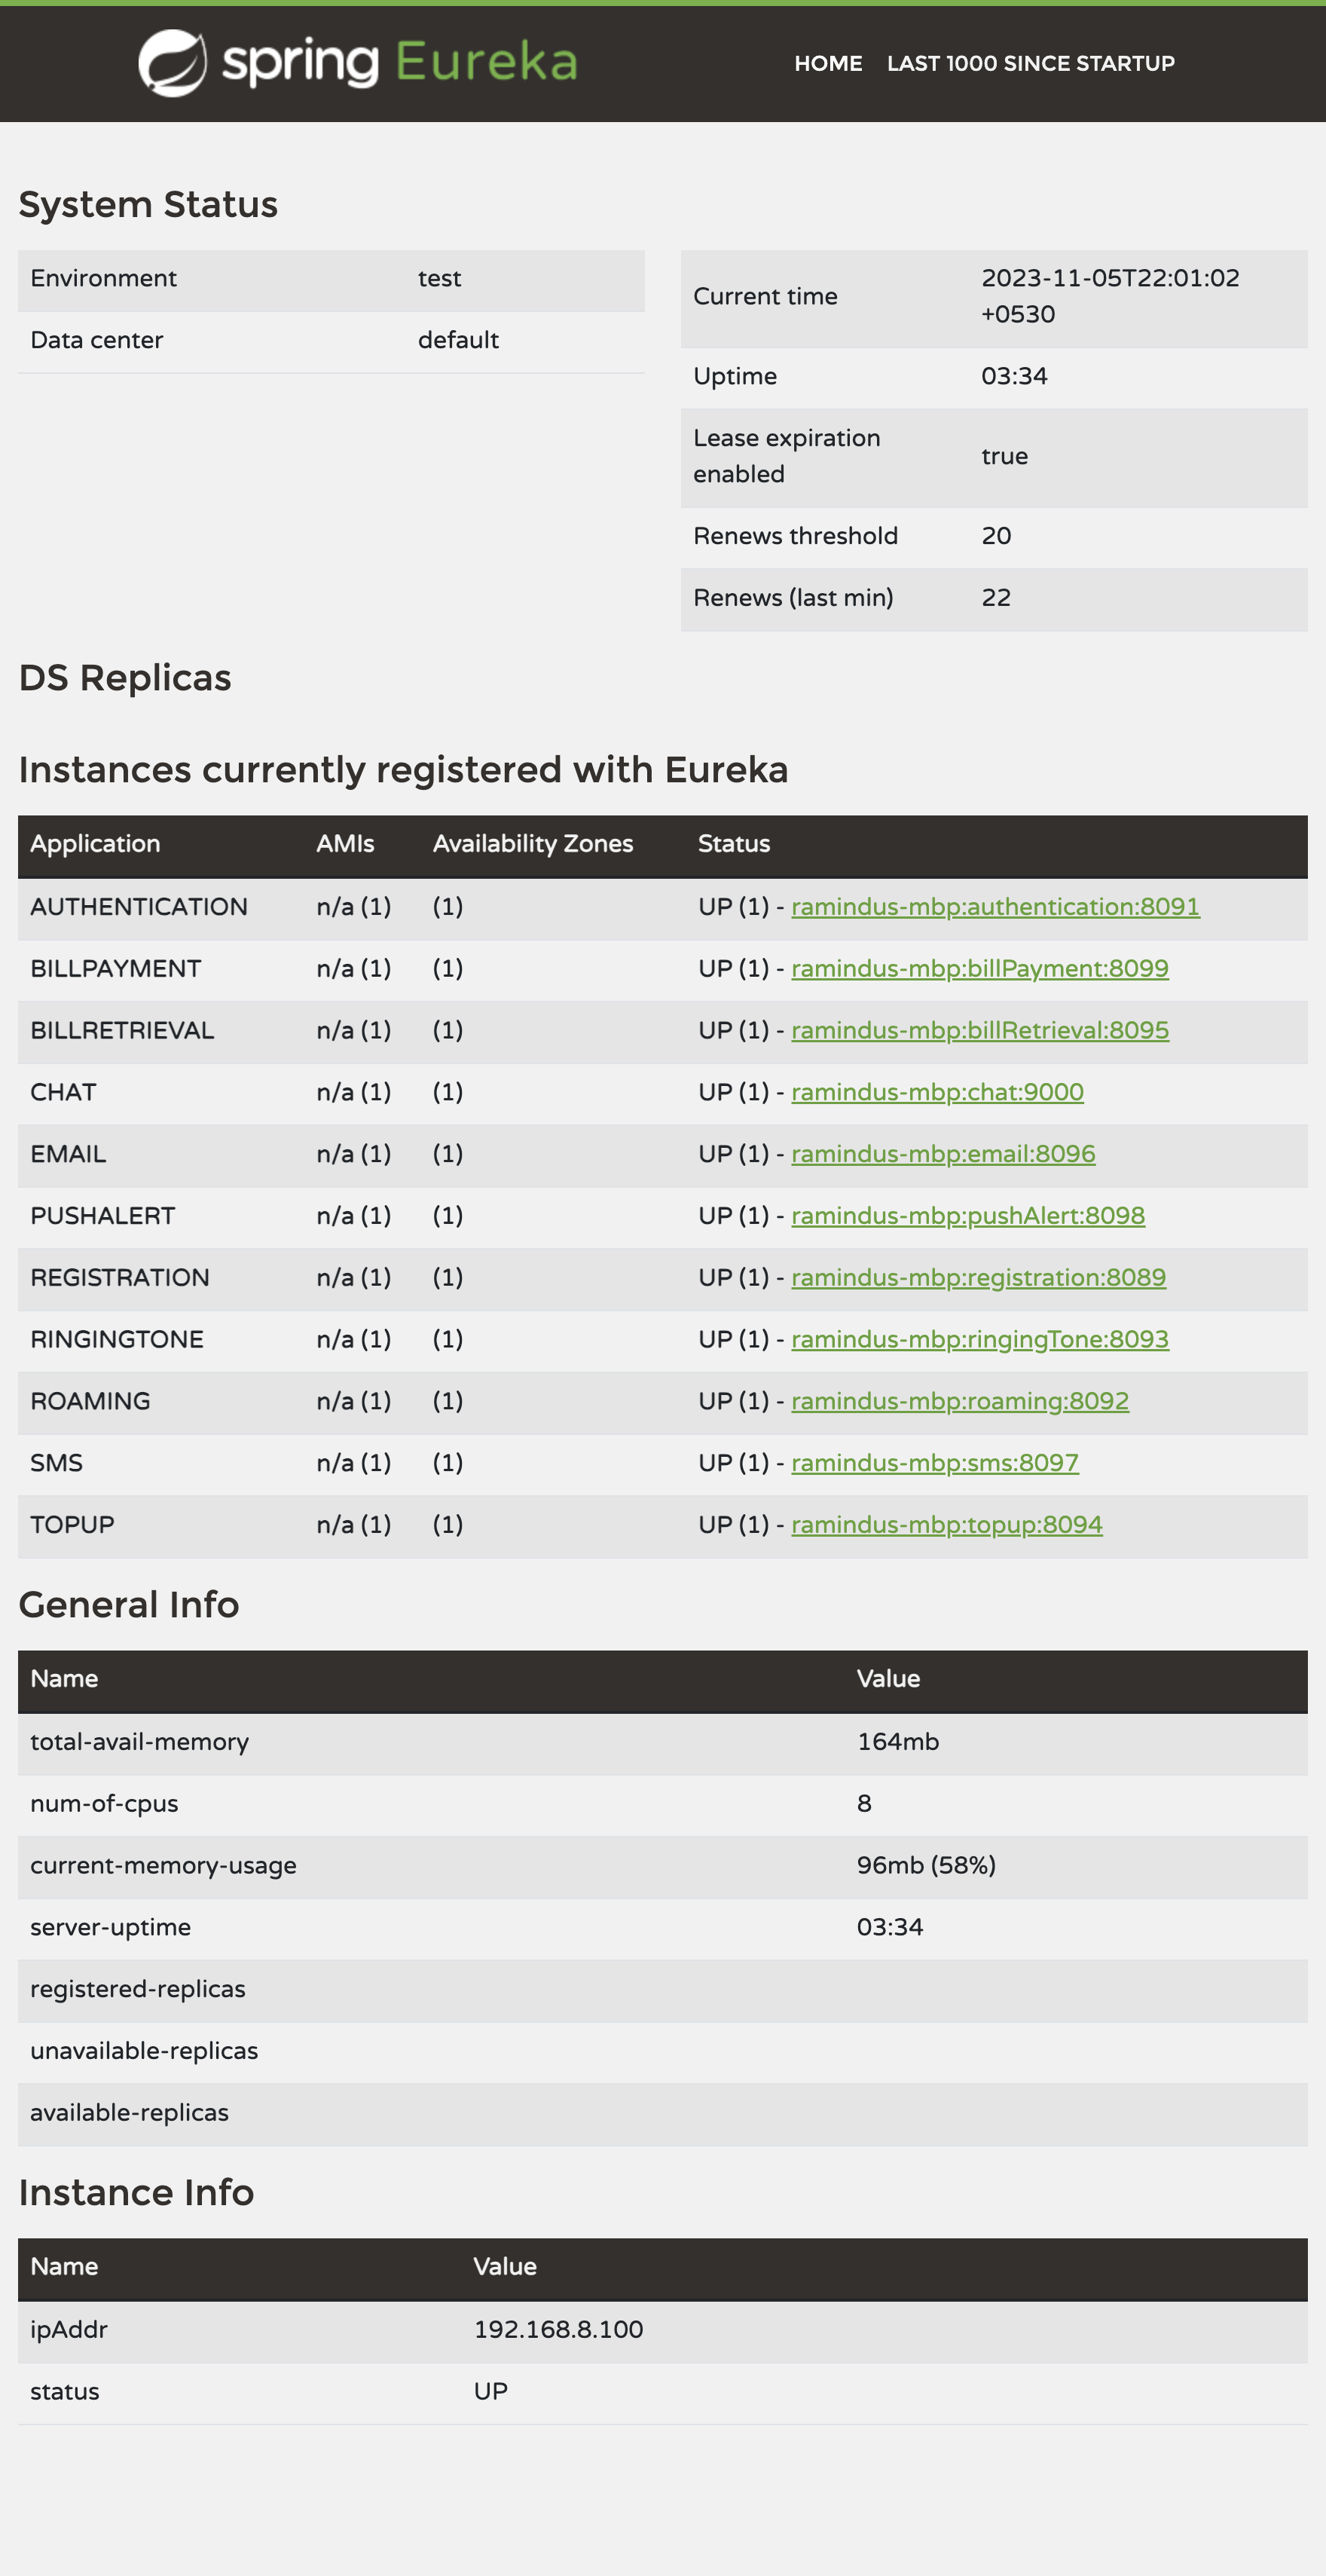
\includegraphics[height=\textheight]{Eureka.png}
    \caption{Eureka Server with all the services running.}
    \label{fig:your-figure-label}
\end{figure}




\section{Implementation Architectures}

The following are two alternative architectures for implementing the solution:

\subsection{Alternative Architecture 1: Monolithic Architecture}
\par In this alternative architecture, the Sri-Tel solution is implemented as a single, tightly integrated monolithic application. All functionalities, including user management, service management, billing, chat support, and external integrations, are bundled into a single codebase and deployed as one application.
\par Monolithic architectures are easier to develop and maintain, as there's no need to manage multiple microservices. In some cases, a monolithic architecture may result in lower latency as there are no network calls between microservices.
\par But, Monolithic applications can be challenging to scale horizontally because all components are tightly coupled and as the application grows, maintaining and updating the monolith becomes more complex. Also Changes in one part of the application may affect other parts, making it less modular. Because of these drawbacks the micro services architecture was selected for the implementation. 

\subsection{Alternative Architecture 2: Service-Oriented Architecture (SOA)}
\par In the SOA architecture, the Sri-Tel solution is designed as a collection of loosely coupled, independent services. Each service focuses on a specific set of functionalities, such as user management, billing, chat support, and external integrations. These services communicate with each other through standardized interfaces, such as APIs or message queues.
\par SOA allows for loose coupling between services, making it easier to update and maintain individual components without impacting the entire system. Also The  services can be reused across different applications or platforms, improving efficiency and reducing development time. SOA supports horizontal scalability as services can be deployed independently based on demand.
\par But in SOA architecture, managing a large number of services and their interactions can become complex and Depending on the implementation, there might be some latency in service-to-service communication.Also SOA requires strong governance to ensure consistency and compatibility among services. As a result of these drawbacks, the microservices architecture was used for the implementation. 



\section{Architectural Patterns and Integration Patterns}
\par The Sri Tel solution is based on a Microservices Architecture implemented using Spring-Boot. The Microservice Architecture divides the application into smaller, loosely coupled services that can be developed, deployed, and maintained independently as the development team of this project follows. It aligns with the requirement to provide distinct functionalities to Sri-Tel users while maintaining agility and scalability as mentioned in the previous section.

\subsection{Integration Patterns}
\begin{itemize}
    \item \textbf{Message-Oriented Integration} 
        This pattern is foundational to the scenario as it involves using messages for communication and integration between different parts of the system. Messages are crucial for sending notifications, alerts, and communication between components.
    \item \textbf{Request-Reply Pattern}
        This pattern is applied in cases where synchronous interactions are necessary, in requesting bill information and verifying payment status with the Payment Gateway.
    \item \textbf{Multiple Consumers}
        This pattern may apply when multiple consumers (customers) receive and process messages, alerts, or chat messages.
    \item \textbf{Return Address}
        Return addresses are used to specify where response messages should be sent in request-reply interactions, ensuring that responses are routed back to the correct recipients.
    \item \textbf{Multiple Service Providers}
        In the context of the Sri-Tel solution, Provisioning System and Payment Gateway, are involved in providing services and integrating with the system.
    \item \textbf{Content-Based Router}
        This pattern is employed to route messages and notifications based on their content or attributes, ensuring that the right messages reach the right recipients.
\end{itemize}


\subsection{Information Security Considerations}
During the design and implementation of the solution, various information security considerations have been addressed.
\begin{itemize}
    \item Authentication and Authorization
    \item Password Management
    \item Payment Security through Payment 
    \item Notifications are only accessed through user accounts
    \item Microservices are independent    
\end{itemize}


\section{Source Code}
GitHub: \href{https://github.com/raminduw200/sritel-microservice}{Sritel-Microservice}

\end{document}